Distributed systems typically consist of two or more components that communicate \emph{asynchronously} by sending and receiving messages through a network layer~\cite{lamport1978time}. Each component has its own input message queue, and when a message arrives, the component responds by executing an appropriate \emph{message handler}. Such a handler consists of a sequence of program statements that might update the internal state of the component, send a message to another component in the system, or even create an entirely new component.

As an example of a distributed system, Figure~\ref{fig:azurestore} shows the top-level components of Azure Storage vNext, a distributed extent management system for Windows Azure that is used in production inside Microsoft. We will use this system as the main running example in this paper. The system is described in more details in Section~\ref{sec:cases:azurestore}, together with another case study from Microsoft.

Azure Storage vNext consists of multiple extent managers, extent nodes, and network engines that are able to send messages across the network, and enqueue any received messages in the input queue of the corresponding node. Each extent manager is responsible for managing a subset of the extent nodes. Each extent node stores its corresponding extent in a local storage, and sends periodical heartbeats and synchronization messages to the extent manager. When the extent manager receives a synchronization message it is responsible to update extent nodes with the latest extent.

\begin{figure}[t]
\centering
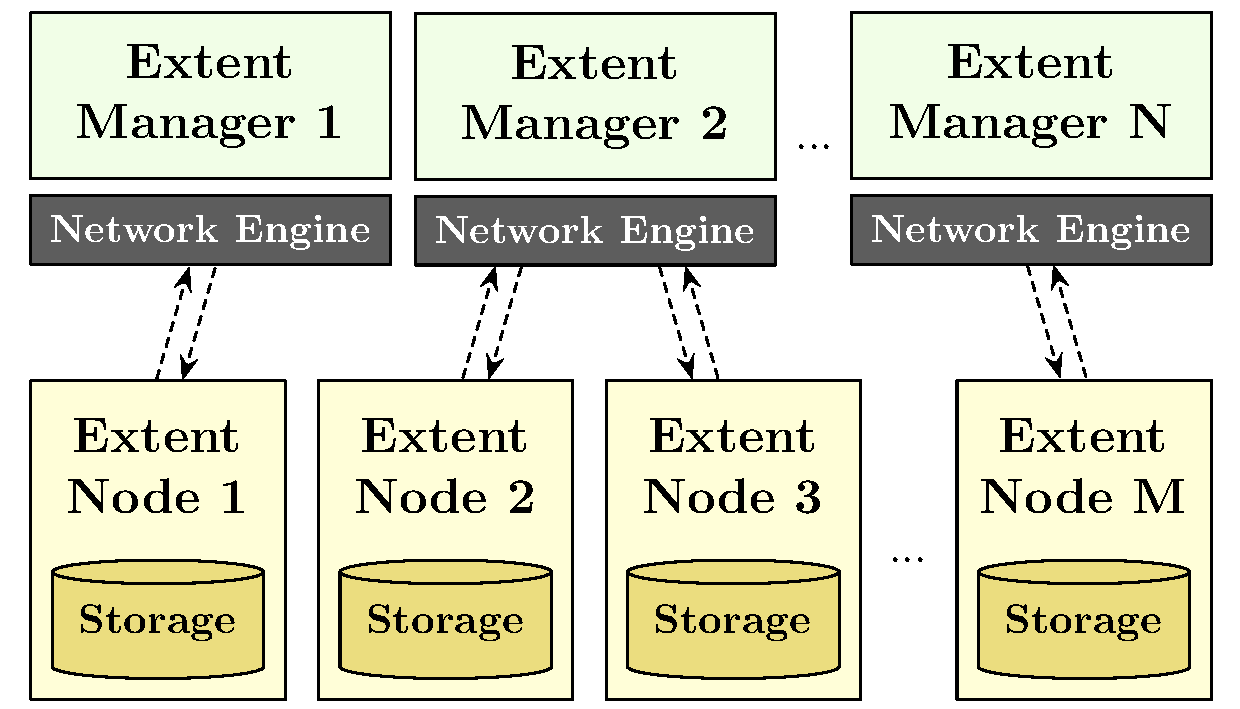
\includegraphics[width=\linewidth]{img/azurestore}
\caption{Top-level components of a distributed extent management system for Windows Azure.}
\label{fig:azurestore}
\end{figure}

\subsection{Bugs in distributed systems}
\label{sec:overview:bugs}

In a distributed system, message handlers can interleave in arbitrary order, because of the asynchronous nature of message-based communication. To complicate matters further, unexpected failures are the norm in production: nodes in a cluster might fail at any moment, and thus programmers have to implement sophisticated mechanisms that can deal with these failures and recover the state of the system. Moreover, with multicore machines having become a commodity, individual components of a distributed system are commonly implemented using multithreaded code, which adds another source of nondeterminism.

All the above sources of nondeterminism (as well as nondeterminism due to timeouts, message losses and client requests) can easily create \emph{heisenbugs}~\cite{gray1986computers, musuvathi2008finding}, which are corner-case bugs that are difficult to detect, diagnose and fix, without using advanced \emph{asynchrony-aware} testing techniques.

We can classify most distributed system bugs in two categories: \emph{safety} and \emph{liveness} property violations~\cite{lamport1977proving}.

\begin{description}
\item[Safety] A safety property checks that an erroneous program state is \emph{never} reached, and is satisfied if it \emph{always} holds in each possible program execution.

\item[Liveness] A liveness property checks that some progress \emph{will} happen, and is satisfied if it \emph{always eventually} holds in each possible program execution.
\end{description}

\noindent
A safety property can be specified using an \emph{assertion} that fails if the property gets violated in some program state. As an example, in Azure Storage vNext we assert that whenever a message gets dequeued there must be an action that can handle the received message. Note that this safety property is not specific to Azure Storage vNext, and can be used in any system based on message passing.

Liveness properties are much harder to specify and check since they apply over entire program executions and not just individual program states. As an example, the liveness property that must be always eventually satisfied in the Azure Storage vNext system is that a user-defined $N$ number of extent nodes must be always eventually available with the latest extent. There was an actual bug in the system, that led this property to fail for some very rare executions. Although this buggy behavior would be observed from time to time during stress testing, there was no way to reproduce the bug. We discuss later in this paper, how we are able to detect and reproduce this bug using our approach.

Normally, liveness checking requires the identification of an infinite fair execution that never satisfies the liveness property~\cite{schuppan2004efficient, musuvathi2008fair}. Prior work~\cite{schuppan2004efficient} has proposed that assuming a program with finite state space, a liveness property can be converted into a safety property. Other researchers proposed the use of heuristics and only exploring finite executions of an infinite state space system using random walks to identify if a liveness property is violated~\cite{killian2007life}.

\PDComment{Quickly say how we found Cheng's bug?}

\subsection{Testing production systems}
\label{sec:overview:testing}

Techniques such as unit testing, integration testing and stress testing are heavily used in industry today for finding bugs in production code. However, these techniques are not effective for testing distributed systems, which have many sources of nondeterminism.

As an example, all the unit test and integration test suites of the Azure Storage vNext project successfully pass every single time. However, the developers found that the stress test suite, which constantly kills and launches extent nodes, could fail from time to time after very long executions. The observed failure was that the liveness property described in Section~\ref{sec:overview:bugs} would not get satisfied. The developers had no way to deterministically reproduce this bug or be able to detect what is the culprit, as the traces they were getting were very long and hard to parse.

The ideal testing technique should be able to work on unmodified distributed systems, capture and control all possible sources of nondeterminism, systematically inject faults in the right places, and explore all feasible execution paths. However, this is easier said than done when testing production systems.

A completely different approach for reasoning about the correctness of distributed systems is to use formal methods.  A notable example is TLA+~\cite{lamport1994temporal}, a formal specification language that can be used to design and verify concurrent programs via model checking. Amazon recently published an article describing their use of TLA+ in Amazon Web Services to verify distributed protocols~\cite{newcombe2015aws}. A limitation of TLA+, as well as other similar specification languages, is that they are applied on a model of the system and not the actual system. Even if the model is verified, there is no guarantee that the code that will actually execute is free of bugs.

Our goal in this work instead is to \emph{test what is actually being executed}. To achieve this we developed a new software engineering methodology for testing distributed systems, implemented on top of the \psharp framework. The original \psharp framework is explain in Section~\ref{sec:overview:psharp}, while the new approach is explained in Section~\ref{}.

\subsection{The \psharp framework}
\label{sec:overview:psharp}

\psharp~\cite{deligiannis2015psharp} provides an \emph{event-driven asynchronous programming} language and a \emph{systematic concurrency testing} engine for developing highly-reliable distributed systems.

The \psharp language is an extension of \csharp, built on top of Microsoft's Roslyn\footnote{\url{https://github.com/dotnet/roslyn}} compiler, that enables asynchronous programming using communicating state-machines. \psharp machines can interact asynchronously by sending and receiving events,\footnote{We use the word ``event'' and ``message'' interchangeably.} an approach commonly used to develop distributed systems. This programming model is similar to actor-based approaches provided by other asynchronous programming languages (e.g. Scala~\cite{odersky2008programming} and Erlang~\cite{armstrong1996erlang}).

A \psharp machine consists of an input event queue, states, state transitions, event handlers, fields and methods. Machines run concurrently with each other, each executing an event handling loop that dequeues an event from the input queue and handles it by invoking an appropriate event handler. This handler might update a field, create a new machine, or send an event to another machine. In \psharp, a send operation is non-blocking; the message is simply enqueued into the input queue of the target machine, and it is up to the operating system scheduler to decide when to dequeue an event and handle it. All this functionality is provided in a lightweight runtime library, build on top of Microsoft's Task Parallel Library~\cite{leijen2009tpl}.

Because \psharp is built on top of \csharp, the programmer can blend \psharp and \csharp code; this not only lowers the overhead of learning a new language, but also allows \psharp to easily integrate with legacy code. Another advantage is that the programmer can use the familiar programming and debugging environment of Visual Studio.

A key capability of the \psharp runtime is that it can run in \emph{bug-finding mode}, where a embedded systematic testing engine captures and takes control of all sources of nondeterminism (such as event handler interleavings, failures, and client requests) in a \psharp program, and then systematically explores all possible executions to discover bugs.

\psharp is available as open-source\footnote{\url{https://github.com/p-org/PSharp}} and is currently used by various teams in Microsoft to develop and test distributed protocols and systems.

\PDComment{Do we want to actually mention (and compare with) P in this paper?}
%The \psharp language belongs to the same family of languages as P~\cite{desai2013p}.
